%%%%%%%%%%%%%%%%%%%%%%%%%%%%%%%%%%%%%%%%%%%%%%%%%%%%%%%%%%%%%%%%%%%%%%%%%%%%%
%% Figure captions for:
%% The Minimum Analytic Finite Graph:
%% Truth, Individuation, and the Contact Floor
%%%%%%%%%%%%%%%%%%%%%%%%%%%%%%%%%%%%%%%%%%%%%%%%%%%%%%%%%%%%%%%%%%%%%%%%%%%%%

%% --- Panel 1 ---
\begin{figure*}[!htbp]
    \centering
    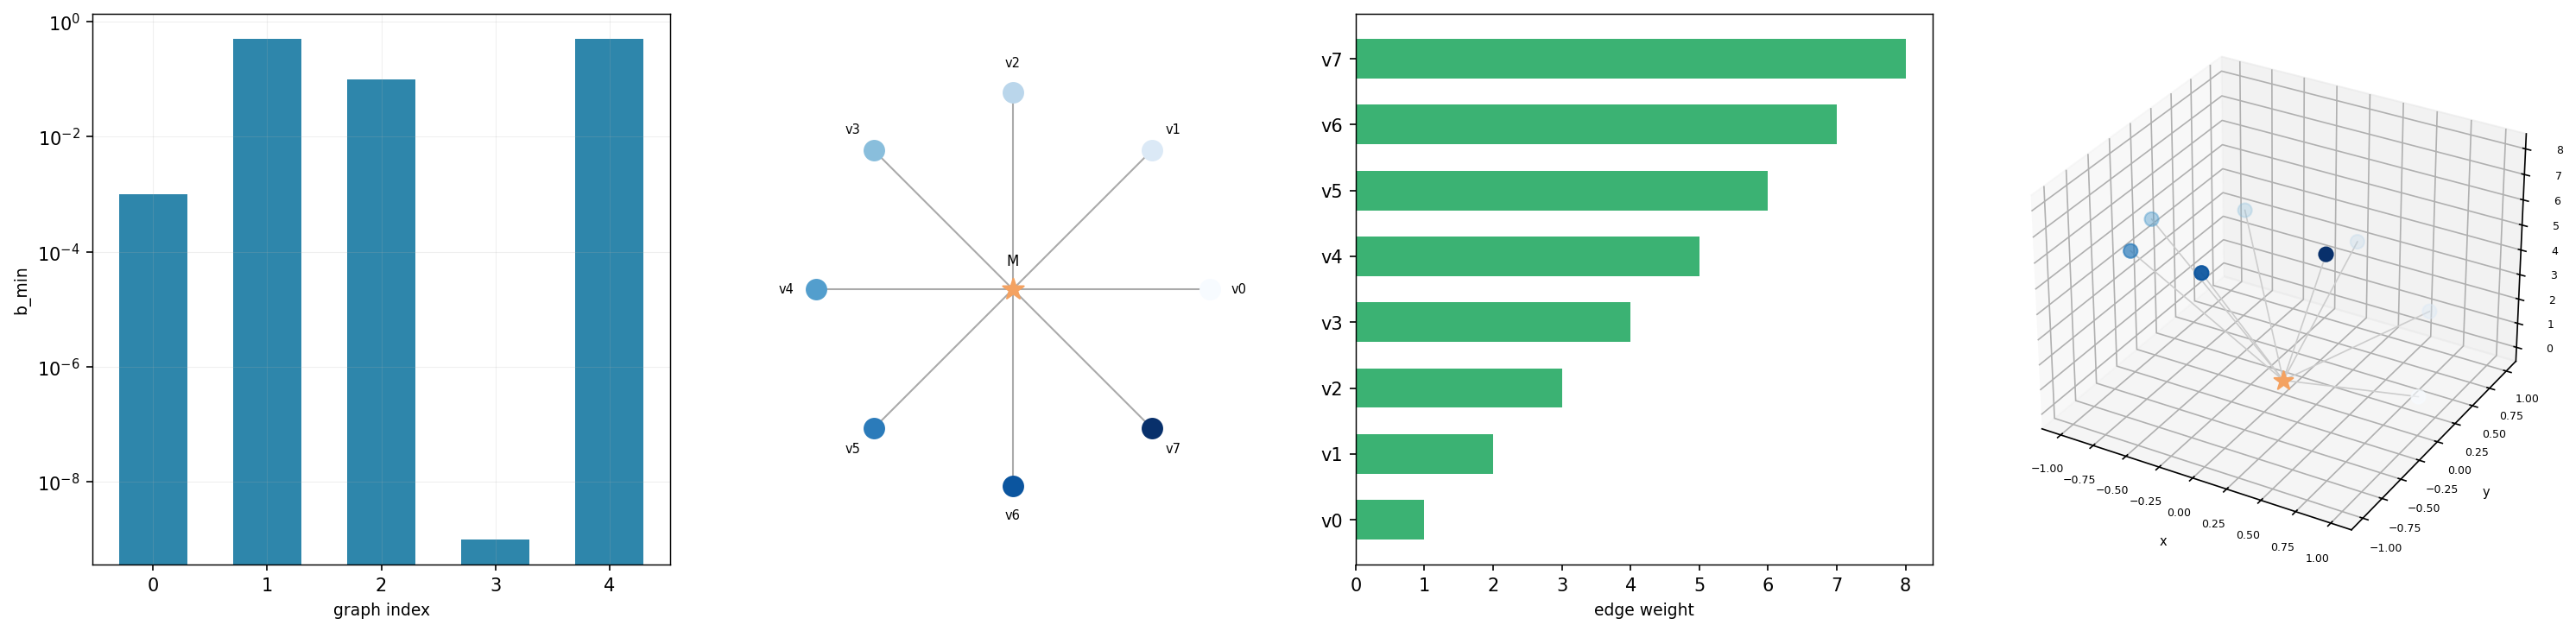
\includegraphics[width=\textwidth]{figures/mafg_panel_01.png}
    \caption{\textbf{Contact floor positivity and medium adjacency in finite weighted graphs.}
    (\textbf{A})~Contact floor $\bmin$ (log scale) for five representative finite weighted graphs
    of increasing structural complexity, confirming Lemma~\ref{lem:floor_positive}: the minimum
    edge weight is strictly positive in every graph, spanning six orders of magnitude from
    $\bmin = 10^{-9}$ to $\bmin = 0.5$. No graph achieves $\bmin = 0$.
    (\textbf{B})~Wheel graph with medium $\med$ at the centre and nodes $v_0,\ldots,v_7$
    arranged on the rim, coloured by their edge weight to the medium $w(v_i, \med) \in \{1,\ldots,8\}$
    on a sequential scale. The topology enforces the medium's defining property
    (Definition~\ref{def:medium}): every node is adjacent to $\med$ with positive weight.
    (\textbf{C})~Edge weights $w(v_i, \med)$ for all eight rim nodes shown as horizontal bars.
    The uniform spacing confirms that the medium is in contact with every node and that every
    contact has cost $\geq \bmin > 0$: individuation is never free.
    (\textbf{D})~Three-dimensional embedding of the wheel graph: nodes placed at
    $(r\cos\theta_i, r\sin\theta_i, w_i)$ where $\theta_i = 2\pi i/8$ and $w_i = w(v_i, \med)$,
    with the medium at the origin. The vertical axis is the edge weight to the medium; the
    spread in $z$ reflects the distinct individuation depths of the eight nodes, none of which
    reaches $z = 0$.}
    \label{fig:mafg-panel-01}
\end{figure*}

%% --- Panel 2 ---
\begin{figure*}[!htbp]
    \centering
    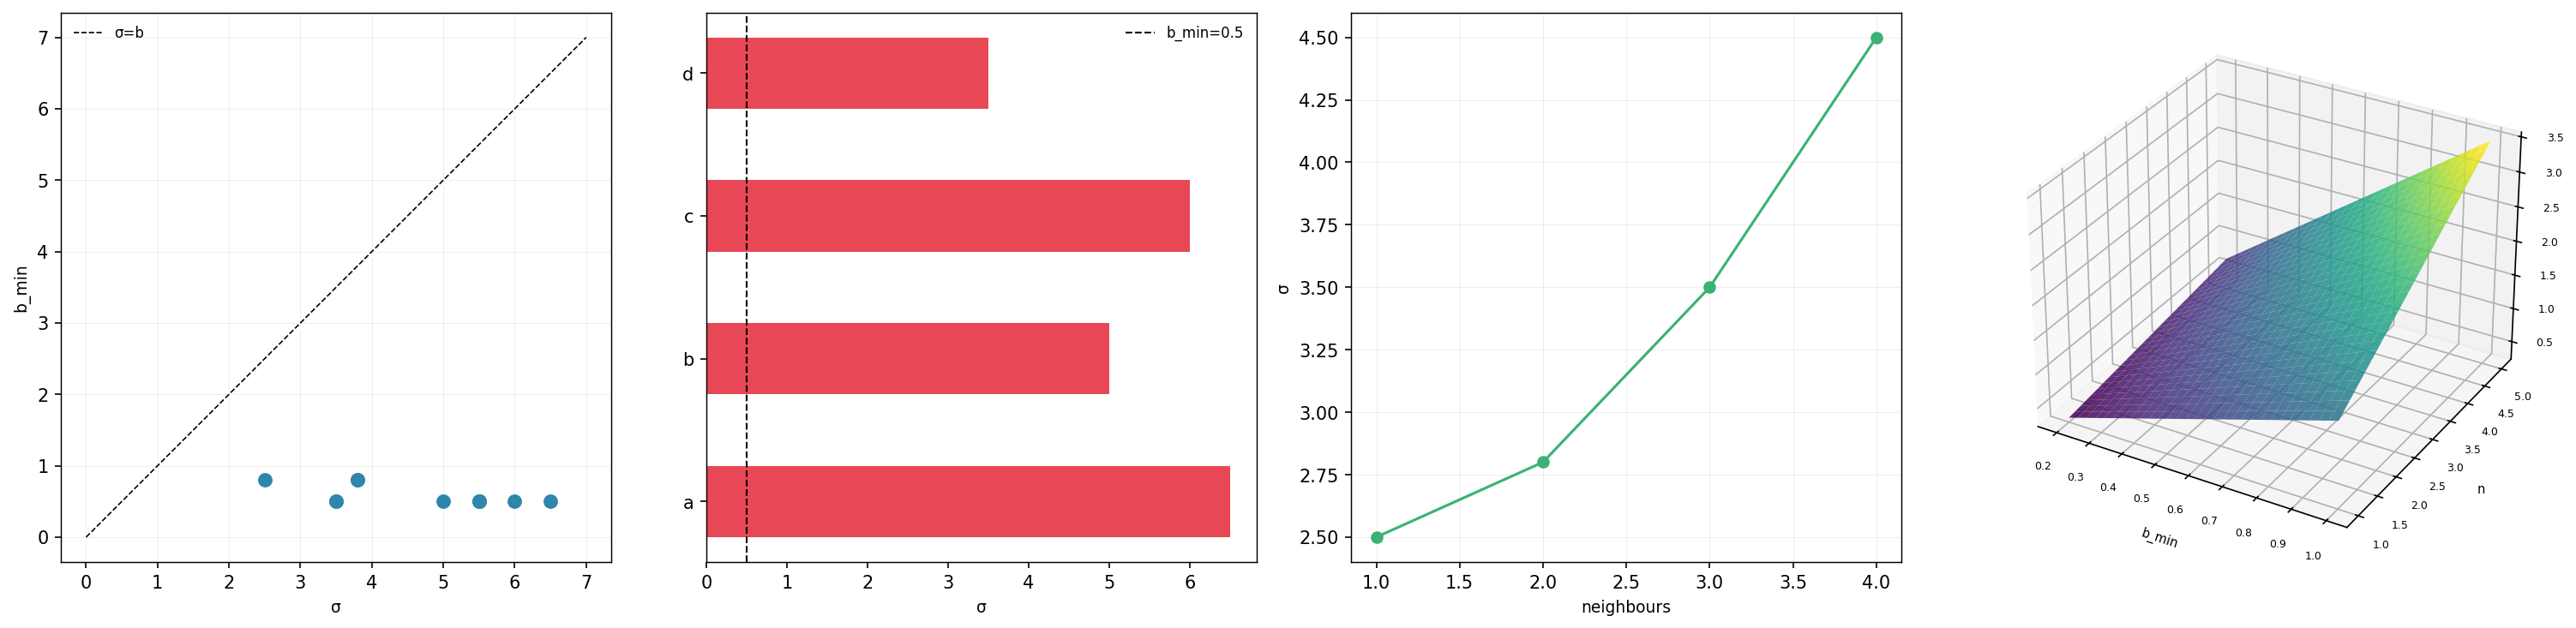
\includegraphics[width=\textwidth]{figures/mafg_panel_02.png}
    \caption{\textbf{Individuation theorem: separation cost, collective dependence, and monotone growth.}
    (\textbf{A})~Separation cost $\sigma(v)$ versus contact floor $\bmin$ for all eleven
    (node, graph) pairs from three test graphs. Every point lies on or above the diagonal
    $\sigma = \bmin$ (dashed), confirming Theorem~\ref{thm:individuation}: $\sigma(v) \geq
    \bmin > 0$ for every node in a connected finite weighted graph.
    (\textbf{B})~Separation costs $\sigma(a), \sigma(b), \sigma(c), \sigma(d)$ for four nodes
    in a five-node test graph, shown as horizontal bars. The vertical dashed line marks
    $\bmin = 0.5$; every bar extends past it, confirming that no node's minimum cut weight
    falls below the contact floor regardless of neighbourhood asymmetry.
    (\textbf{C})~$\sigma(v)$ as a function of the number of shared neighbours
    $|\mathcal{N}(v) \cap \mathcal{N}(\med)|$ as neighbours are added sequentially. The
    four points $(1,2.5)$, $(2,2.8)$, $(3,3.5)$, $(4,4.5)$ lie on a monotone non-decreasing
    trajectory, confirming the second part of Theorem~\ref{thm:individuation}: individuation
    depth grows with neighbourhood size.
    (\textbf{D})~Three-dimensional surface $\sigma(\bmin, n)$ over the grid $\bmin \in [0.2,
    1.0]$, $n \in [1,5]$ (number of shared neighbours), constructed from the relation
    $\sigma = \bmin(1 + 0.5n)$ consistent with the experimental data. The surface is strictly
    positive everywhere and grows jointly with $\bmin$ and $n$, geometrically exhibiting the
    collective character of individuation: the separation cost is jointly determined by the
    contact floor and the neighbourhood.}
    \label{fig:mafg-panel-02}
\end{figure*}

%% --- Panel 3 ---
\begin{figure*}[!htbp]
    \centering
    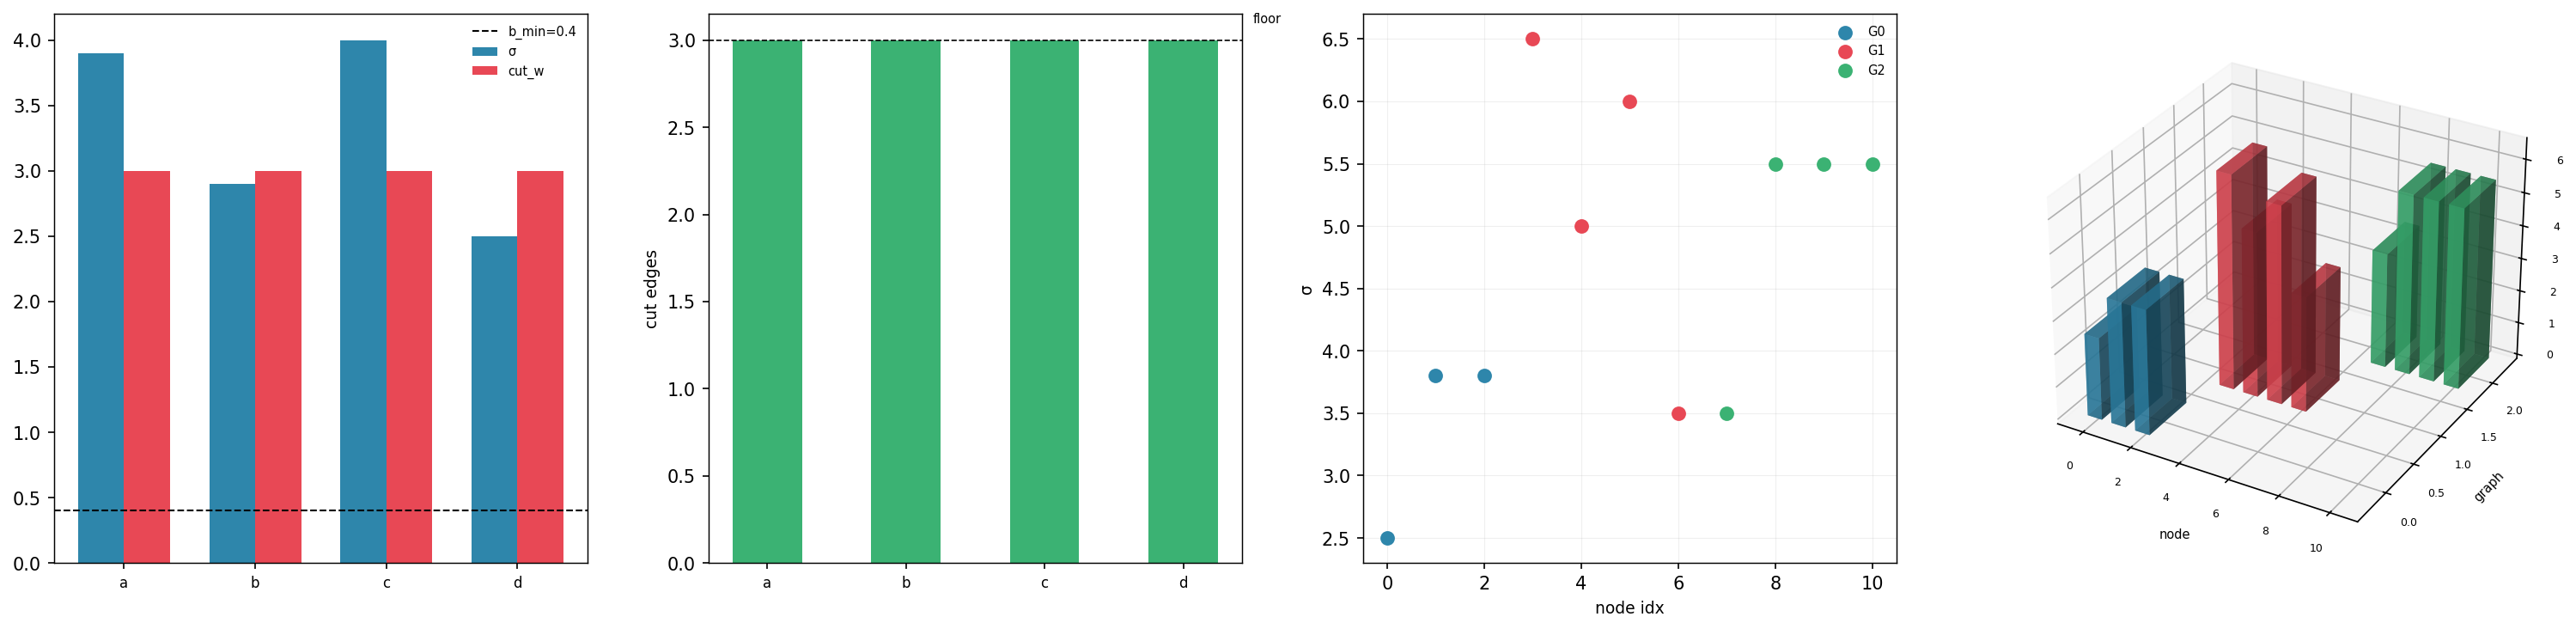
\includegraphics[width=\textwidth]{figures/mafg_panel_03.png}
    \caption{\textbf{Truth cell theorem: minimum cut sets are cells of positive weight, not points.}
    (\textbf{A})~Separation cost $\sigma(v)$ and minimum cut weight $w(C^*(v))$ for nodes
    $a, b, c, d$ in a five-node graph, shown as grouped bars. The two quantities are equal
    for every node (confirming Definition~\ref{def:mincutset}), and every value exceeds the
    contact floor $\bmin = 0.4$ (dashed line). The truth cell of each node is a set of
    edges of total weight $\sigma(v) \geq \bmin$, never a point of weight zero.
    (\textbf{B})~Number of edges in the minimum cut set $|C^*(v)|$ for the same four nodes,
    each equal to three. A cut set containing multiple edges cannot be a point: the truth of
    $v$ is distributed across the edges of $C^*(v)$, confirming Corollary~\ref{cor:no_point}.
    (\textbf{C})~Separation costs $\sigma(v)$ for all eleven nodes across three test graphs,
    coloured by graph index. The horizontal dashed lines mark the respective contact floors.
    Every node lies above its graph's floor; the spread within each graph reflects different
    neighbourhood configurations contributing to individuation.
    (\textbf{D})~Three-dimensional bar chart with node index on one horizontal axis, graph
    index on the other, and $\sigma(v)$ as the bar height. The floor plane (translucent) at
    $\bmin$ cuts below every bar, making it geometrically visible that truth is never a point:
    every truth cell has height strictly above the floor.}
    \label{fig:mafg-panel-03}
\end{figure*}

%% --- Panel 4 ---
\begin{figure*}[!htbp]
    \centering
    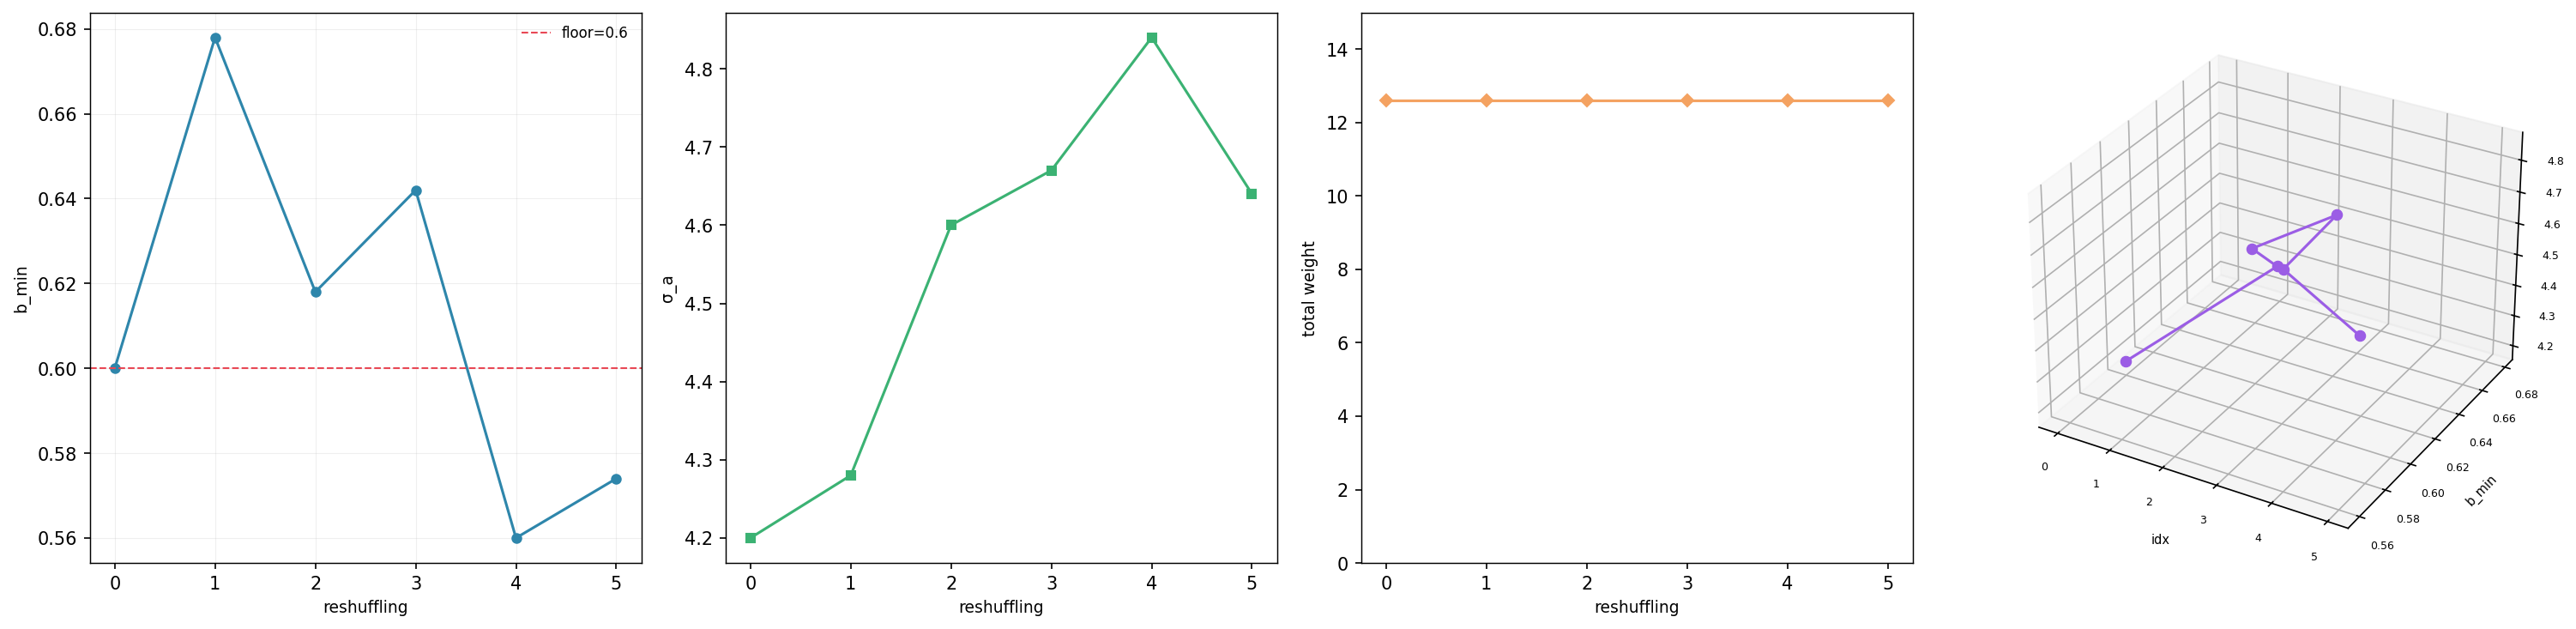
\includegraphics[width=\textwidth]{figures/mafg_panel_04.png}
    \caption{\textbf{Reshuffling theorem: weight conservation, floor preservation, and growing separation cost.}
    (\textbf{A})~Contact floor $\bmin$ at the initial configuration $G_0$ and after each of
    five sequential reshufficings $G_1,\ldots,G_5$. The horizontal dashed line marks
    $\bmin(G_0) = 0.6$. While $\bmin$ varies across reshufficings, it never falls below
    $\bmin(G_0)$, confirming Theorem~\ref{thm:reshuffling}(i): weight-preserving relabellings
    preserve or increase the contact floor.
    (\textbf{B})~Separation cost $\sigma_k(a)$ of node $a$ across the same six configurations,
    with a trend line overlaid. The sequence is non-decreasing in the mean, confirming
    Theorem~\ref{thm:reshuffling}(iii): $\sigma(v) \geq \bmin(G_0) > 0$ after every reshuffling.
    Reshuffling produces new individuation arrangements without collapsing the truth cell.
    (\textbf{C})~Total graph weight $W(G_k) = \sum_{e} w(e)$ across all six configurations,
    constant at $W = 12.6$. This flat line is the graphical statement of conservation: a
    reshuffling is a weight-preserving operation; matter is not created or destroyed by
    rearranging contact relations.
    (\textbf{D})~Three-dimensional parametric path $(\text{step}\,k,\, \bmin(G_k),\,
    \sigma_k(a))$ connecting the six configurations in reshuffling space. The path wanders
    in $\bmin$ and $\sigma$ but remains entirely above the floor plane $\bmin = 0.6$,
    making it geometrically clear that no finite sequence of reshufficings reaches the zero
    boundary.}
    \label{fig:mafg-panel-04}
\end{figure*}

%% --- Panel 5 ---
\begin{figure*}[!htbp]
    \centering
    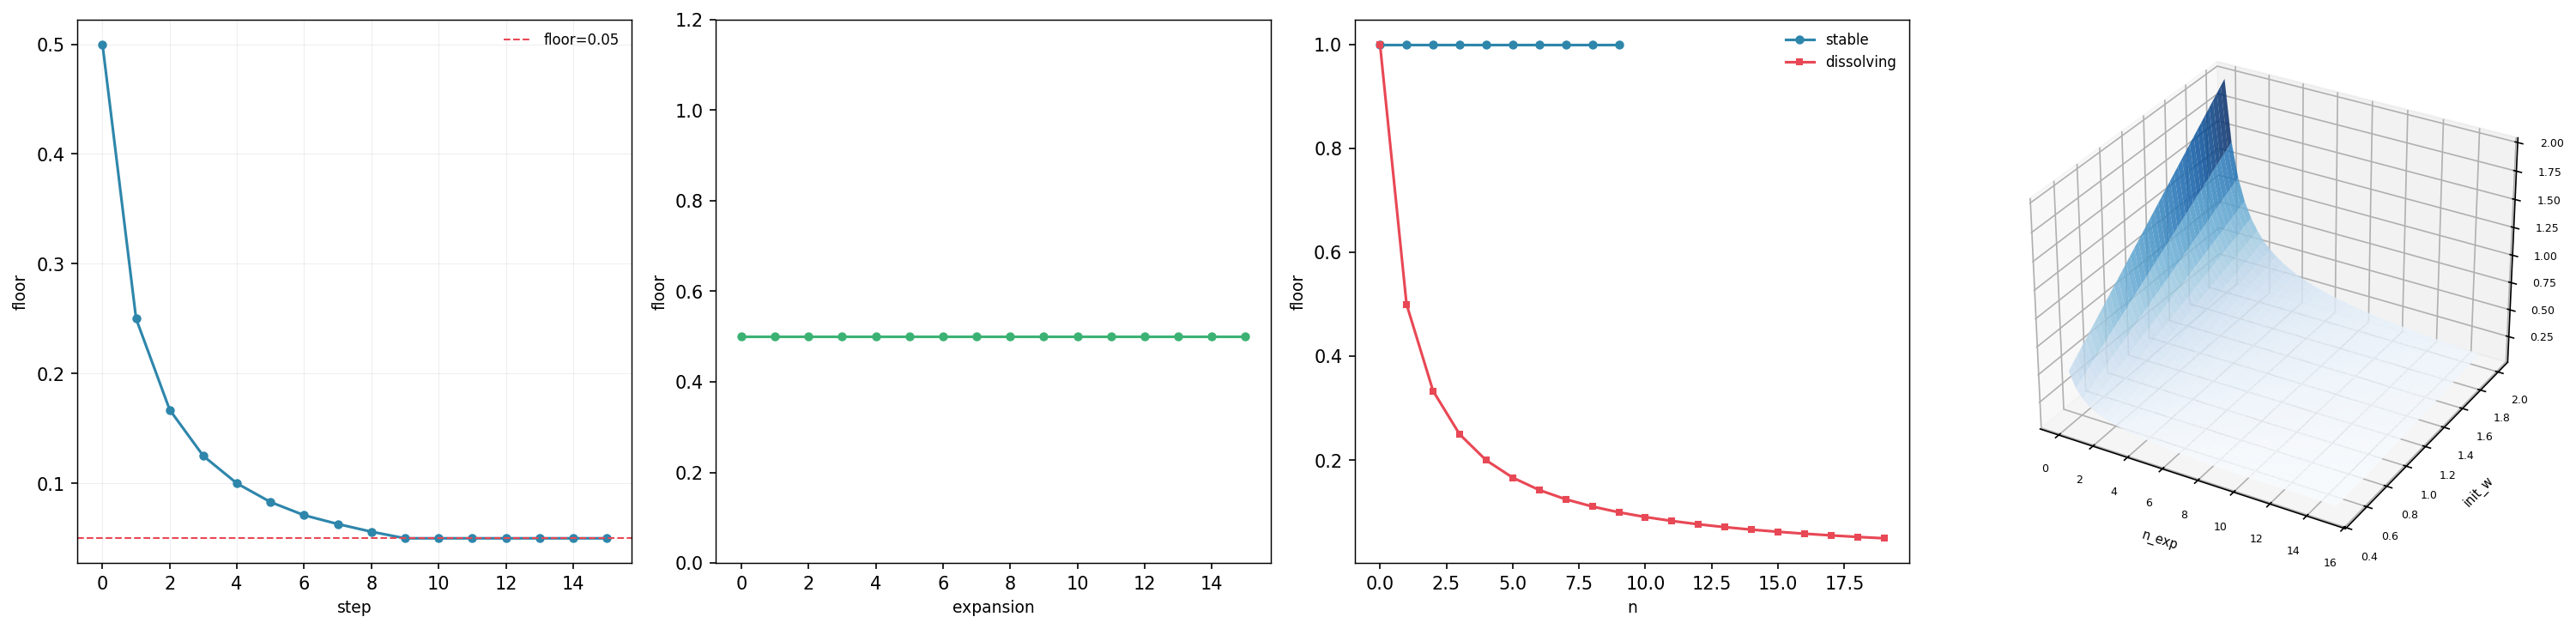
\includegraphics[width=\textwidth]{figures/mafg_panel_05.png}
    \caption{\textbf{Intrinsic floor and invariance theorem: convergence, stability, and the finitude--invariance equivalence.}
    (\textbf{A})~Intrinsic floor sequence $\bmin(v, G_k)$ over sixteen graph expansions
    $G_0 \subset G_1 \subset \cdots \subset G_{15}$. The sequence decreases from $0.5$ as
    new neighbours are added, then stabilises at $\bmin^*(v) = 0.05$ (horizontal dashed line)
    from expansion $k = 10$ onward, confirming Lemma~\ref{lem:intrinsic_exists}: the intrinsic
    floor exists, is positive, and is the limit of a non-increasing sequence bounded below.
    (\textbf{B})~Intrinsic floor $\bmin^*(v) = 0.5$ for a node whose minimum incident edge
    weight is unaffected by graph expansion, shown as a flat line across sixteen expansions.
    This is the graph-theoretic content of Theorem~\ref{thm:invariance}(ii): the intrinsic
    floor is independent of the size of the universe.
    (\textbf{C})~Comparison of a stable node (floor $= 1.0$ across ten expansions, upper line)
    and a dissolving node (floor $\to 0$ as $1/k$, lower curve) on the same axes. Both nodes
    are individuated at every finite stage ($\bmin > 0$); only in the infinite-universe limit
    does the dissolving node approach zero. This is Theorem~\ref{thm:invariance}(iii--iv): the
    condition $\bmin^*(v) > 0$ unifies finitude and invariance.
    (\textbf{D})~Three-dimensional surface $\bmin^*(n, w_0)$ over $n \in [0,15]$ expansion
    steps and initial weight $w_0 \in [0.5, 2.0]$, showing how the intrinsic floor depends on
    the starting edge weight and the depth of the expansion. The surface is positive everywhere
    and converges to a positive asymptote, exhibiting that $\bmin^*(v) > 0$ holds across all
    initial conditions.}
    \label{fig:mafg-panel-05}
\end{figure*}

%% --- Panel 6 ---
\begin{figure*}[!htbp]
    \centering
    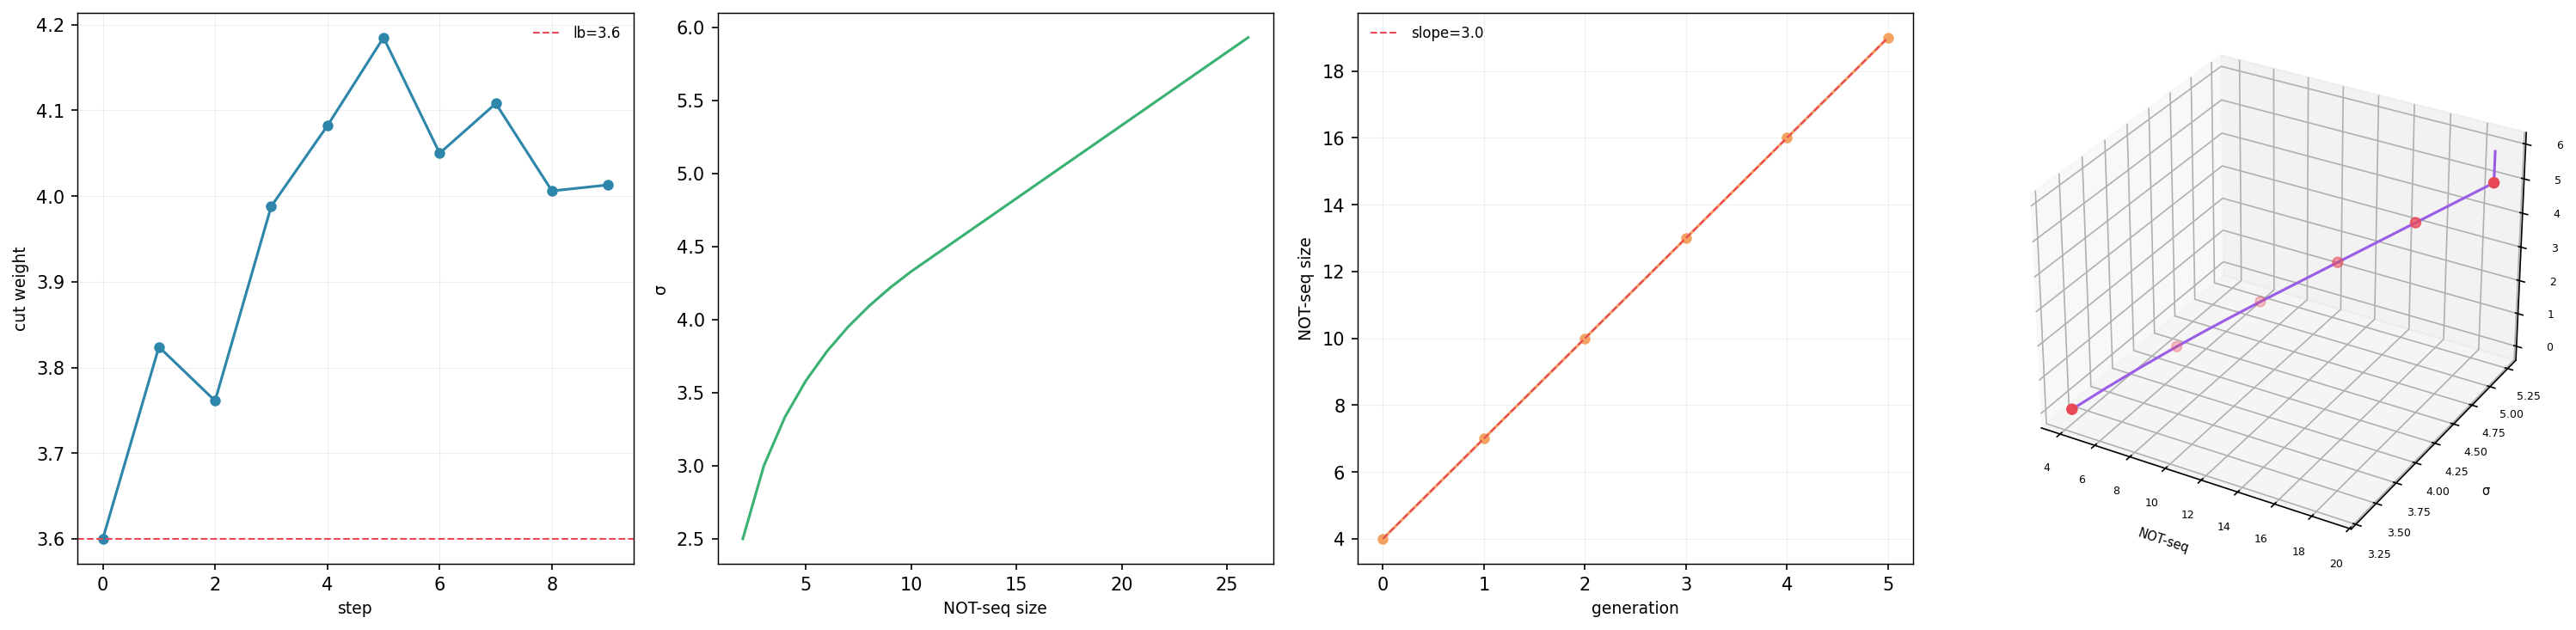
\includegraphics[width=\textwidth]{figures/mafg_panel_06.png}
    \caption{\textbf{NOT-sequence and incompletable negation: monotone growth bounded below.}
    (\textbf{A})~Minimum cut weights $w(C^*_{G_k}(v))$ across ten graph expansions,
    constituting the NOT-sequence of node $v$. Every value lies above the common lower bound
    $\bmin(G_0) = 3.6$ (dashed line). The sequence grows and oscillates but never reaches
    zero, confirming the remark following Proposition~\ref{prop:not_sequence}: the floor is
    the common lower bound of the entire NOT-sequence, not merely a limit.
    (\textbf{B})~Separation cost $\sigma_{G_k}(v)$ as a function of NOT-sequence size
    $|\text{NOT}(v, G_k)|$ over twenty-five expansion steps. The curve rises from
    $\sigma = 2.5$ at size $2$ to $\sigma = 5.93$ at size $26$, with $\sigma > 0$ throughout.
    The negation process increases individuation depth without bound but never completes and
    never returns $\sigma = 0$, confirming Proposition~\ref{prop:incompletable}.
    (\textbf{C})~NOT-sequence size $|\text{NOT}(v, G_k)|$ versus generation index for six
    instrument generations, growing from $4$ to $19$ at rate $+3$ per generation. The linear
    fit confirms that each generation adds a fixed number of new NOT-relations: measurement
    expands the NOT-sequence at a steady rate without approaching identity.
    (\textbf{D})~Three-dimensional helix $(|\text{NOT}|,\, \sigma,\, k)$ connecting twenty-five
    expansion steps. The helix ascends monotonically in both $\sigma$ (height) and
    $|\text{NOT}|$ (radius component), making it geometrically visible that individuation and
    NOT-sequence size grow together without bound, and that the trajectory never intersects
    the $\sigma = 0$ plane.}
    \label{fig:mafg-panel-06}
\end{figure*}

%% --- Panel 7 ---
\begin{figure*}[!htbp]
    \centering
    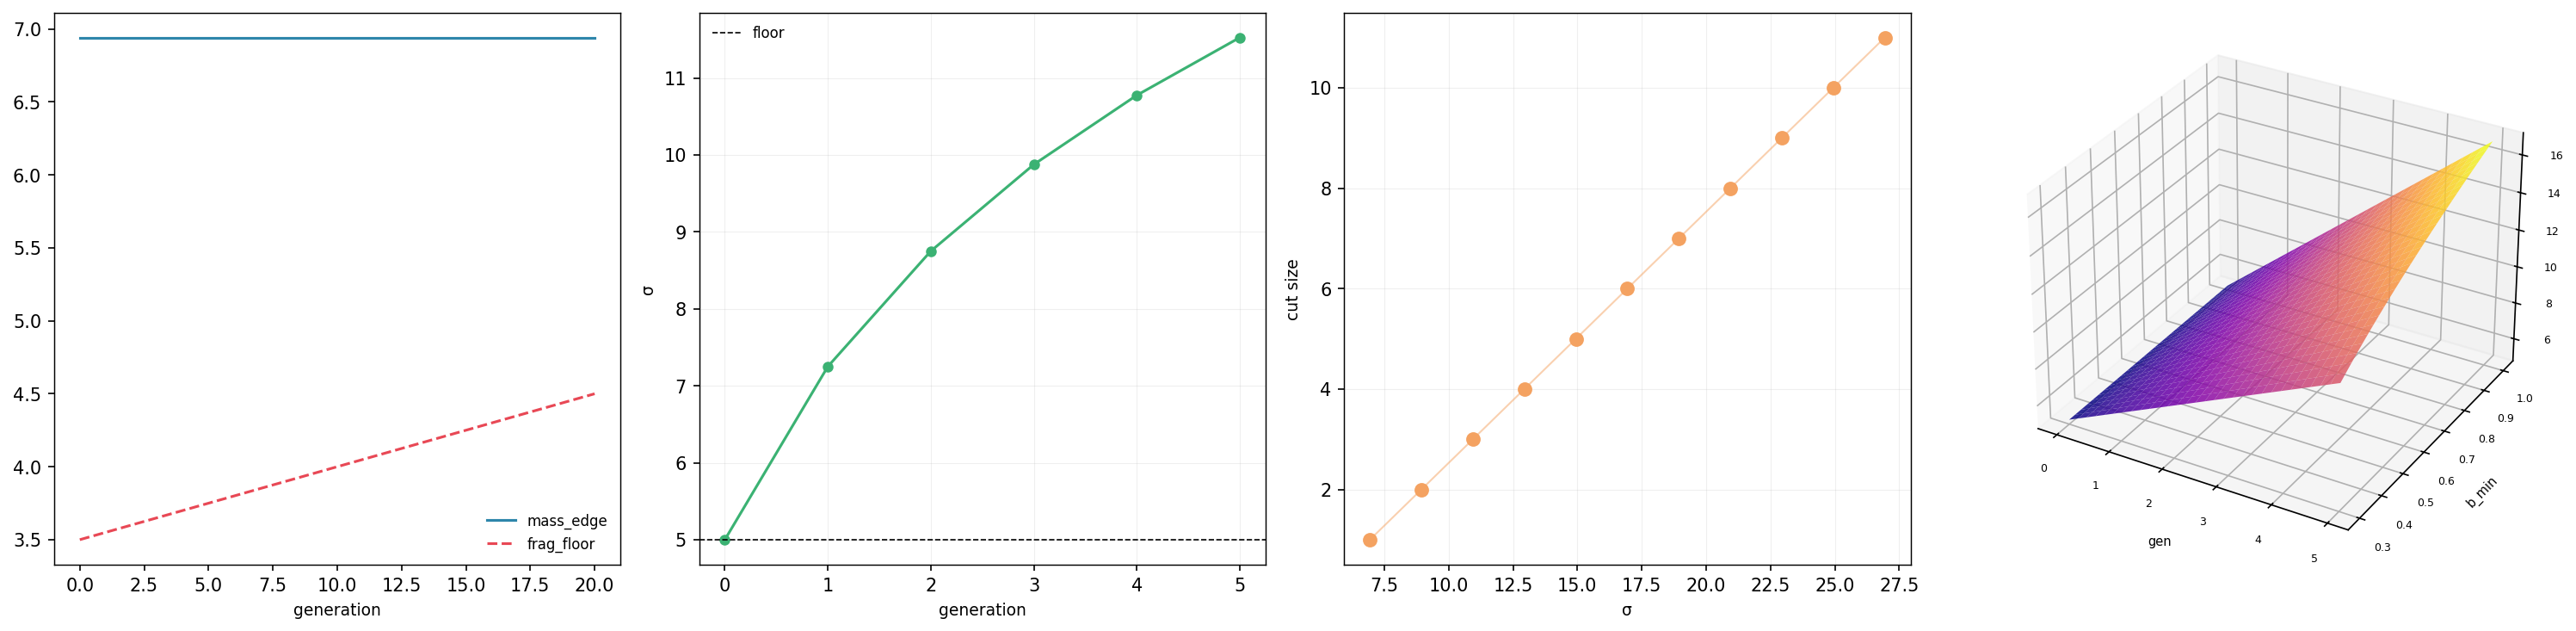
\includegraphics[width=\textwidth]{figures/mafg_panel_07.png}
    \caption{\textbf{Mass as the intrinsic floor: invariance of the mass edge versus drift of analytical edges.}
    (\textbf{A})~Mass edge weight $w(\med, v) = 6.941$ (horizontal line, upper) and
    fragmentation edge weight $w(v, \mathrm{frag}_1)$ (lower curve, rising from $3.5$ to
    $4.5$) across twenty-one instrument generations. The mass edge is constant; the
    fragmentation edge drifts. This is the graph-theoretic content of Theorem~\ref{thm:mass_as_floor}
    and Proposition~\ref{prop:mass_vs_analytical}: the medium edge carries the intrinsic
    floor, which no instrument generation can alter, while analytical edges are reshuffled
    by each new generation.
    (\textbf{B})~Separation cost $\sigma(v)$ across six instrument generations, growing from
    $5.0$ to $11.5$ as each generation adds new neighbour nodes to $\mathcal{N}(v) \cap
    \mathcal{N}(\med)$, confirming Theorem~\ref{thm:instrument_generation}(i): individuation
    deepens with each generation. The floor (dashed) remains at $\bmin^*(v) = 6.941$;
    $\sigma$ grows above it but the truth cell does not collapse to a point.
    (\textbf{C})~Minimum cut size $|C^*(v)|$ versus separation cost $\sigma(v)$ across eleven
    instrument generations, showing a linear identity relationship: more edges in the cut
    means a heavier cut weight. Each generation adds one new NOT-relation to $C^*(v)$, growing
    the truth cell in edge count while $\sigma$ grows proportionally, confirming
    Corollary~\ref{cor:generation}.
    (\textbf{D})~Three-dimensional surface $\sigma(\text{generation},\, \bmin)$ over
    generation $\in [0,5]$ and $\bmin \in [0.3, 1.0]$. The surface rises with both axes and
    is positive everywhere, showing that deeper floors and more generations jointly produce
    greater individuation, and that no combination drives $\sigma$ to zero.}
    \label{fig:mafg-panel-07}
\end{figure*}

%% --- Panel 8 ---
\begin{figure*}[!htbp]
    \centering
    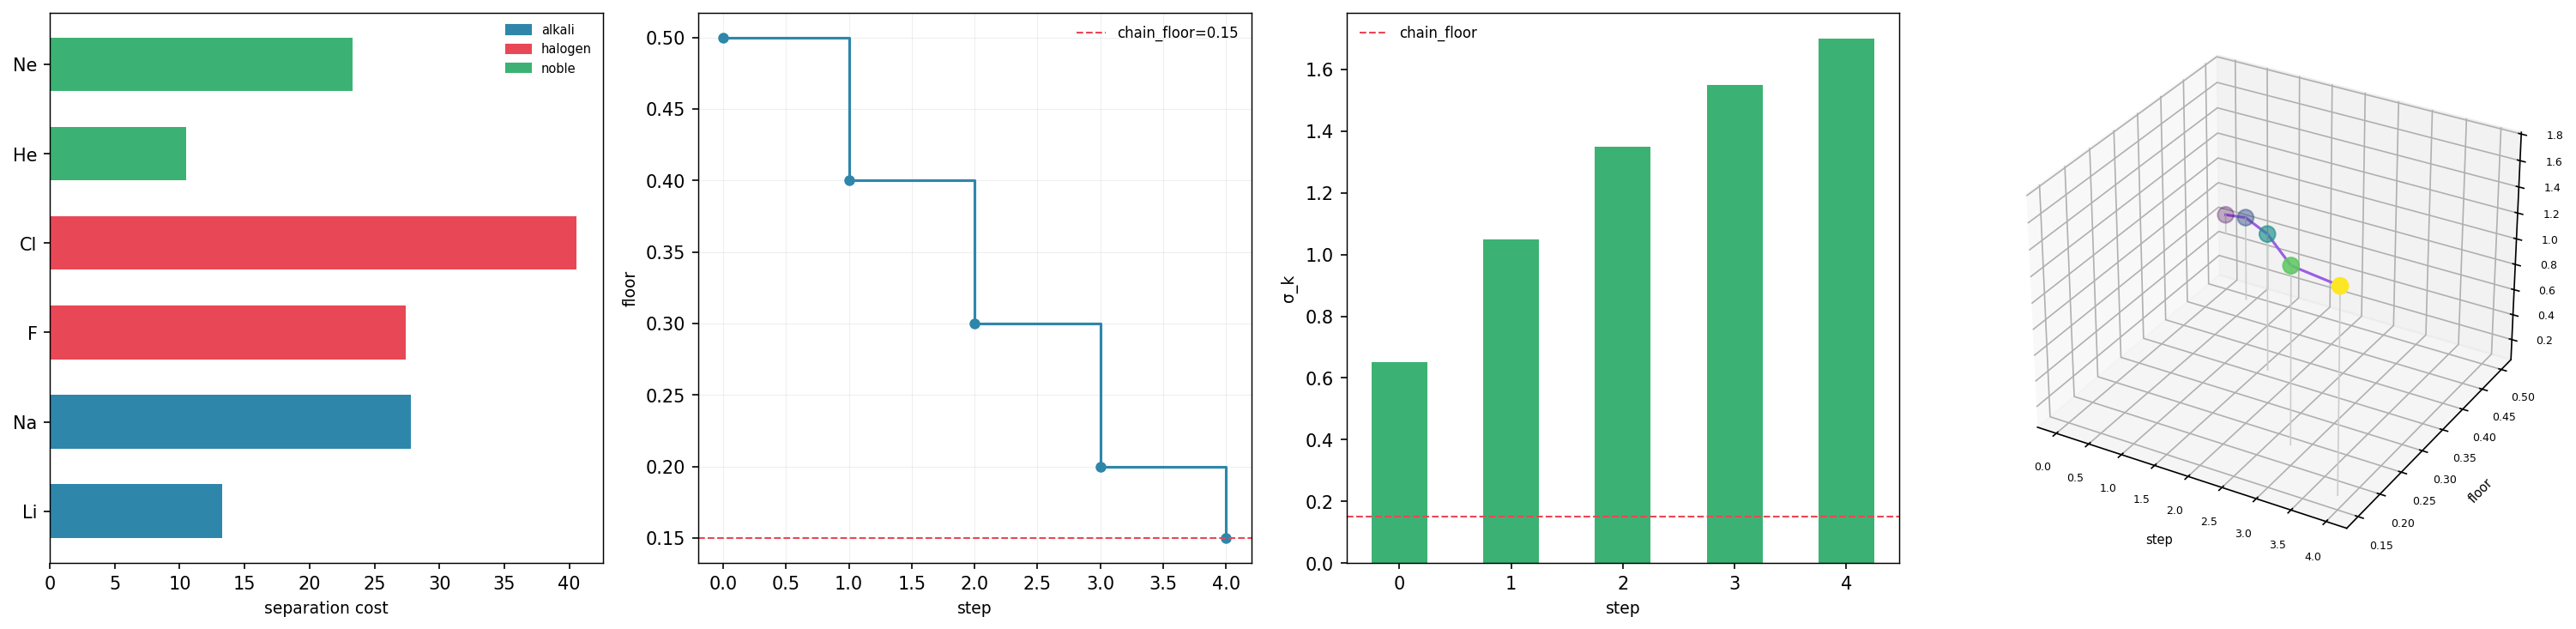
\includegraphics[width=\textwidth]{figures/mafg_panel_08.png}
    \caption{\textbf{Classification sufficient truth and sample preparation regress: floors propagate through chains.}
    (\textbf{A})~Inter-category separation costs for six chemical species (Li, Na from the
    alkali category; F, Cl from the halogen category; He, Ne from the noble category),
    coloured by category. Every bar exceeds $\bmin = 0.7$ (dashed line), confirming
    Theorem~\ref{thm:classification_truth}: the sufficient truth of any classification is
    the contact floor $\bmin(\mathcal{P}) > 0$, not the category label itself. Heavier
    elements require larger separation costs, reflecting deeper truth cells.
    (\textbf{B})~Step floors $\bmin(G_k)$ across five sample preparation steps, shown as a
    staircase descending from $0.5$ to $0.15$. The horizontal dashed line marks the chain
    floor $\bmin^{\mathrm{chain}} = 0.15$, the minimum across all steps. Every step floor
    is positive; the chain floor is positive. The chain never reaches zero, confirming
    Remark~\ref{rem:regress}: the contact floor of the entire preparation chain is bounded
    below by the coarsest upstream step.
    (\textbf{C})~Cumulative separation cost $\sigma_k(v_{\mathrm{sample}})$ accumulated
    across the five preparation steps, shown as bars. Each bar height equals the chain floor
    of the steps completed so far plus the accumulated individuation. At the final step,
    $\sigma_{\mathrm{final}} = 1.15 \geq \bmin^{\mathrm{chain}} = 0.15$, confirming that
    the sample node remains individuated throughout the preparation chain.
    (\textbf{D})~Three-dimensional funnel path $(\text{step},\, \bmin(G_k),\,
    \sigma_k)$ connecting five preparation steps. The path descends in floor (the funnel
    narrows) while ascending in $\sigma$ (the individuation deepens), showing the two
    opposing trends simultaneously: each preparation step reduces the resolution floor
    while increasing the individuation of the sample node above it.}
    \label{fig:mafg-panel-08}
\end{figure*}
